\chapter{Initial experiments} % (fold)
\label{cha:experiments}

In this chapter we present initial experiments to show advantages of our proposal.
First we present case study to show the high convergence of BA.

\section{Bacteriological algorithm convergence}

The first case study aims to show the high convergence of BA. We ran our solution
in Hadoop standalone mode. The test consisted in running the BA with the wordcount job
that calculated the frequency that occur in the input files.

The test was configured with a population of size 3, i.e. with three set of knobs
per generation, each set of knobs had 10 knobs. The input files were generated with
Hadoop job called {\it randomtextwriter} generating 10GB of random text file. The
sample percent was of 10 percent of the input, i.e. 1GB of data.

We ran the BA in three rounds, up to three generations, up to six generations and
last one up to ten generations. The input set of knobs for the first round was
generated randomly, after for the next round the set of knobs were the best three
of the previous round. So, ocurring feedback of the process.

In Fig.~\ref{fig:3gen} the first round started with three random set of knobs, we can
see the progress in 3 generations resulting an improvement almost of 3\% better
than the first generation.
\\
\begin{figure}[htbp]
    \centering
	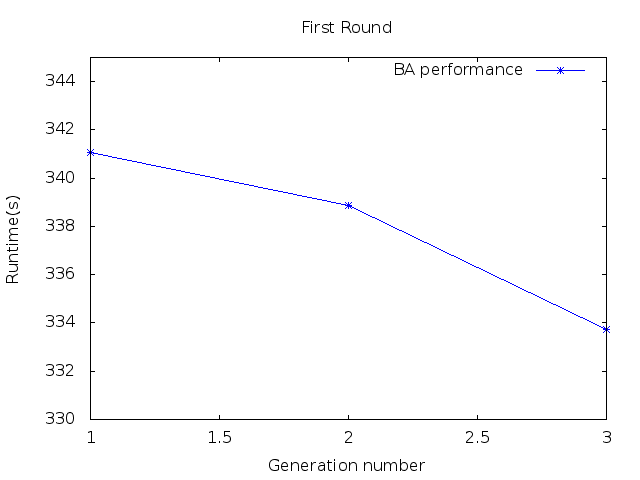
\includegraphics[scale=0.6]{graphics/img/3gen.png}
    \caption{First round up to 3 generations} \label{fig:3gen}
\end{figure}
\\
\\

In Fig.~\ref{fig:6gen} the second round started with the best three set of knobs
of the first round. We can see the two first generations were worse than the best
result of the last round, this occured because greater usage of the cluster. However,
from the third generation the performance improved and the resulting was better
in 16\%.
\\
\\
\begin{figure}[htbp]
\begin{center}
	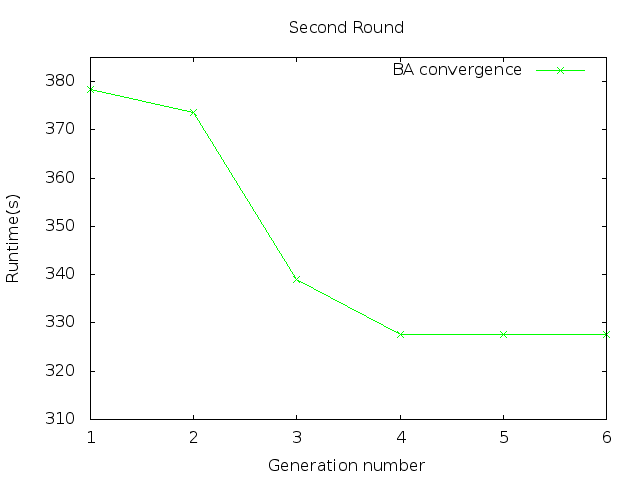
\includegraphics[scale=0.6]{graphics/img/6gen.png}
\caption{Second round up to 6 generations} \label{fig:6gen}
\end{center}
\end{figure}
\\
\\
\\
\\
\\
\\
\\
\\
\\
\\
\\
\\
\\
\\
\\
\\
\\

In Fig.\ref{fig:10gen} the third round started  with the best three set of knobs
of the second round. In this round we can realize the biggest drop of the runtime.
It started with the same time of the best set reached in the second round,
as the BA runs the runtime improves until stabilization in the final generations.
This improvement occurred because some knobs values representing input, merge and
sort buffers were changed, occurring further adjustment to the cluster. 
\\
\begin{figure}[htbp]
\begin{center}
	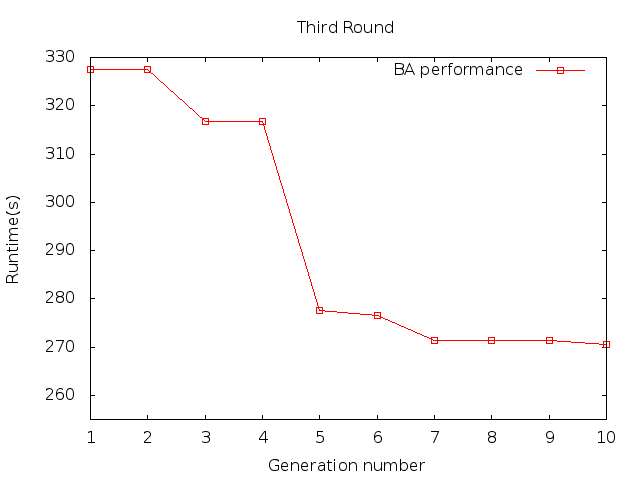
\includegraphics[scale=0.7]{graphics/img/10gen.png}
\caption{Third round up to 10 generations} \label{fig:10gen}
\end{center}
\end{figure}
\\

With these three figures \ref{fig:3gen}, \ref{fig:6gen} and \ref{fig:10gen}
we can realize as the generations progress the runtime
never recede, i.e. the runtime of one generation is lower or equal than the
previous generation. This occurs because of the memorization operator
avoids regressions in the BA performance.
\\
\\
\\
\\
\\
\\
\\
\\
\\

\begin{figure}[htbp]
\begin{center}
	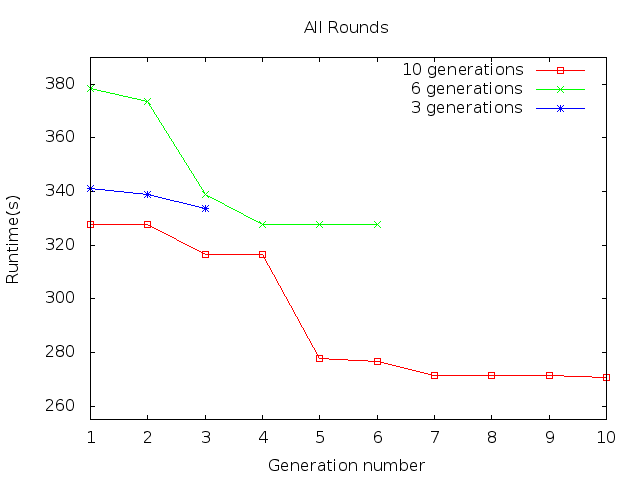
\includegraphics[scale=0.6]{graphics/img/all.png}
\caption{All Rounds} \label{fig:allgen}
\end{center}
\end{figure}

Figure \ref{fig:allgen} is an aggregation of all the rounds. It aims
to show the overall improvement of the runtime. The first set of knobs reached
the runtime of 380 seconds in the first round, and the last set of knobs reached
the runtime of 270 seconds in the last round. The overall improvement was about
30~\% which is a considerable improvement.

Moreover, the result were influenced by the feedback provided by the software
between the rounds. So, as the rounds progress the improvement continue occurring
influenced by the feedback operator.
